\documentclass{report}
\usepackage{amsmath} 
\usepackage{hyperref}
\usepackage{graphicx}
\graphicspath{ {images/} }

\title{UTA Method}
\author{Elie Daher}

\begin{document}
\pagenumbering{gobble}
\maketitle
\abstract This report contains the summary of the chapter \textbf{UTA Methods} from the Book: Multiple Criteria Decision Analysis. This document was made during my internship at LAMSADE in the summer of 2017.
\tableofcontents{}
\pagenumbering{arabic}

\chapter{Introduction}
In decision theory a basic problem involving several criterias, concerns the way that the final decision should be made. However, this problem is posed in the opposite way: assuming that the decision is given, how is it possible to find the rational basis for the decision being made? Or how is it possible to assess the model leading to exactly the same decision as the actual one or the most "similar" decision.\\

The following steps represent the methodology of decision-making problems: 
\begin{enumerate}
\item object of the decision, definition of the set of potential actions and the determination of a problem statement
\item modeling a consistent family of criteria
\item defining a global preference model
\item decision-aid or decision support
\end{enumerate}

\underline{Example: Buying a new car} \\

Let's consider we are trying to figure out which car to buy. Using the methodology represented above, we state that the objective of this problem is \textbf{buying a new car}. After stating the objective, we can list the potential of actions that represent the list of cars that we may buy: 
\begin{itemize}
\item Peugeot 208 GTi
\item Nissan Sentra
\item Citroen C4
\item Peugeot 308 berline
\end{itemize}
After listing the list of potential cars, we can define a list of criteria that we will base our decision on. When defining the list of criteria you should always remember that the potential actions should be evaluated by those criterias, so the criteria must be easy to evaluate and should be logical. Let's say we will base our purchase on the following criteria:
\begin{itemize}
\item price (in Euro)
\item comfort (0, +, ++, +++) \textit{0 being not comfortable and +++ very comfortable}
\item safety (1, 2, 3, 4, 5) \textit{1 being not safety and 5 safe}
\end{itemize}
During the decision process, we will determinate the global preferences of the potential actions:
\begin{enumerate}
\item Citroen C4
\item Peugeot 208 GTi
\item Peugeot 308 berline
\item Nissan Sentra
\end{enumerate}
Once the global preference is defined, we can start the decision support.\\

In this document, we will study a multi-criteria decision analysis mehtods UTA, a method proposed in 1982 that build a utility function based on the preference of the DM. More precisely we will conduct our research over the new version of UTA: UTASTAR. The method is illustrated on an example.

\chapter{UTA Method}
One of the multi-criteria decision analysis methods is the UTA method, which was proposed by E. Jacquet-Lagrèze and J. Siskos in 1982. This method is proposed by the Multi-Attribute Utility Theory (MAUT) that build a utility function based on the DM\footnote{Decision Maker} preferences.\\
 
The UTA method is used to solve a multi-criteria problem by building a utility function based on the preferences of the DM and solving a linear program (LP). It adopt the aggregation-disaggregation principles: where the model is based on a given preferences.\\

The UTASTAR has been considered a better algorithm than UTA. Better result were found using the UTASTAR algorithm. So this is why we will focus on this method rather than the UTA method.\\

At the begining of the problem, the DM should present the following information 
\begin{itemize}
\item rank of the actions
\item give the criteria he want to base his decision on 
\item evaluate the action compared to the criterion
\end{itemize}
Once those information are presented, the UTASTAR algorithm can be executed. 

\newpage
\section{Principles and Notation}
Let's call $A={a,b,c,...}$ the set of potential actions and $g_1, g_2, g_3, ..., g_n$ the family of criteria. Where $g_i(a)$ represent the funtion of an action(alternative)$a$ on the criteria $g_i$ with $a \in A_R$. \\

We define $g_{i*}$ as the least preferred criteria: $g_{i*} = min_{a \in A} g_i (a)$ and $g_i^{*}$ as the most preferred criteria: $g_i^{*} = max_{a \in A} g_i (a)$. So the interval for each criteria $g_i$ is: $[g_{i*} , g_i^{*}]$.\\

If we want to evaluate two actions, for example $a$ and $b$, on only one criteria $g_i$ we have the following relations: 
\begin{equation}
      \begin{cases}
      	a \succ b\Leftrightarrow g_i(a) > g_i(b) \quad preference\\
      	a\sim b \Leftrightarrow g_i(a) = g_i(b) \quad indifference \\
      \end{cases}
\end{equation}
The criteria aggregation model in UTA has the following form:
\begin{equation}\label{eq1}
      v(g(a)) = \sum_{i=1}^{n} v_i (g_i (a))
\end{equation}
subject to normalization constraints:\\
\begin{equation}\label{eq2}
      \begin{cases}
      	\sum_{i=1}^{n} v_i(g_{i}^{*}) = 1\\
       	v_i(g_{i*})= v_i(g_i^1)  = 0,  \forall i = 1, 2, ..., n\\
      \end{cases}
\end{equation}
where $ v_i, i = 1,2,...,n$ are non decreasing real valued function.\\

In UTASTAR we have 
\begin{equation}
	w_{ij} = v_i(g_i^{j+1}) - v_i(g_i^{j}) \geq 0 \quad \forall i \quad j 
\end{equation}

Which will allow us to write: 
\begin{equation}
	v_i(g_i^j) =	  \sum_{t=1}^{j-1} w_{it} \quad \forall i = 1,2,...,n \quad and \quad j = 2,3,...,\alpha _i -1 \\
\end{equation}

With the evaluation of an action a $g(a) = [g_1(a) ,  g_2(a) , ... , g_n(a)] $, we have the following relation:
\begin{equation}
      \begin{cases}
      	v[g(a)] > v[g(b)] \Leftrightarrow a \succ b\\
      	v[g(a)] \sim v[g(b)] \Leftrightarrow a = b\\
      \end{cases}
\end{equation}

\newpage
\section{Development} 
The updated version of UTA, UTASTAR, propose a double error function for each action: $\sigma ^{+} (a)$ and $\sigma ^{-} (a)$.  So the value of each alternative $a \in A_R$ can be written: \\
\begin{equation}
	v^{'} [g(a)] = \sum_{i=1}^{n} v_i [g_i (a)] - \sigma ^{+} (a)+ \sigma ^{-} (a) \quad  \forall a \in A_R
\end{equation}
\begin{center}
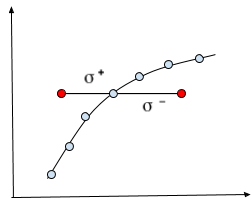
\includegraphics{error-function-utastar}
\end{center}

For each criteria, the interval $[g_{i*}, g_i^{*}]$ is cut into $(\alpha _i -1)$ equals interval, and the end points $g_i^{j}$ are given by the formula:
\begin{equation}
	g_i^{j}= g_{i*} + \frac{j-1}{\alpha _i -1} (g_i^{*} - g_{i*})  \forall j = 1,2, ..., \alpha _i
\end{equation}

The marginal value of an action $a$ is calculated by a linear interpolation
\begin{equation}
	v_i [g_i (a)] = v_i (g_i^{j}) + \frac{g_i (a) - g_i^{j}}{ g_i^{j+1} - g_i^{j}} [v_i (g_i^{j+1}) - v_i (g_i^{j}) ] 
\end{equation}

The set of reference action $ A_R = a_1, a_2, ... , a_m$ is arranged where $a_1$ is the best action and $a_m$ is the worst action. Which indicate that we have two possible situations:
\begin{itemize}
\item $a_k  \succ a_{k+1} \quad $ preference 
\item $a_k \sim a_{k+1} \quad $ indifference
\end{itemize} 

So if we have that $\Delta (a_k, a_{k+1} ) = v^{'} [g(a_k)] - v^{'} [g(a_{k+1})]$ and $\delta$ is a small positive number we will obtain the following relations: 
\begin{equation}\label{eq3}
      \begin{cases}
      	\Delta (a_k, a_{k+1} ) \geq \delta\\
       	\Delta (a_k, a_{k+1} ) = 0 \\
      \end{cases}
\end{equation}
The marginal value functions are estimated by means of the Linear Programm with \eqref{eq1}, \eqref{eq2}, \eqref{eq3} as constraints, and an objective function depending on the $ \sigma^{+}$ and $\sigma^{-} $: 
$$ [min]z = \sum_{k=1}^{m} [ \sigma ^{+} (a_k) + \sigma ^{-} (a_k)]  $$
subject to: 
\begin{equation}\label{eq5}
      \begin{cases}
      	\Delta (a_k, a_{k+1} ) \geq \delta \quad or \quad \Delta (a_k, a_{k+1} ) = 0 \\
      	\sum_{i=1}^{n} \sum_{j=1}^{\alpha_i -1} w_{ij} = 1\\
       	w_{ij} \geq 0, \quad \sigma^{+}(a_k) \geq 0, \quad \sigma^{-}(a_k) \geq 0, \quad  \forall i, j  and  k\\
      \end{cases}
\end{equation}

\chapter{Example}
working on it

\chapter{Conclusion}
The UTA method build a utility function based on the preferences of the DM and it consist in solving a linear program (LP) to solve a multi-criteria problem.\\

This method will elaborate a model of preferences which is as similiar as possible to the DM's preferences.\\

An improved version of the UTA is the UTASTAR. In UTA we used a single error $\sigma(a)$ in UTASTAR we use a double positive error function. The updated version has performed better than the regular method.

\begin{thebibliography}{9}
\bibitem{latexcompanion} Salvatore Greco, Matthias Ehrgott, Jose Rui Figueira \textit{Multiple Criteria Decision Analysis}. State of the Art Surveys, 2004.
\bibitem{utastar} Siskos, Yannacopoulos \textit{UTASTAR: an ordinal regression method for building additive value functions}
\bibitem{cahier24} Siskos \textit{Cahier du LAMSADE: Les programmes UTA}, 1979
\bibitem{theseAHammami} Abdelkader Hammami, These du grade Philosophiae Doctor PHD de la Faculte des Sciences et de Genie \textit{Modelisation Technico-Economique d'une chaine logistique dans une entreprise reseau}, 2003
\end{thebibliography}

\end{document}